%%----------------------------------------------------------------------------80
%% Preamble
%%----------------------------------------------------------------------------80
\documentclass[10pt,aspectratio=96]{beamer}
\usepackage[some]{background}
\usepackage[T1]{fontenc}
\usepackage{amsmath}
\usepackage{appendixnumberbeamer}
\usepackage{array}
\usepackage{booktabs}
\usepackage{colortbl}
\usepackage{fontawesome}
\usepackage{geometry}
\usepackage{graphicx}
\usepackage{hologo}
\usepackage{lipsum}
\usepackage{multirow}
\usepackage{pdflscape}
\usepackage{pgfcalendar}
\usepackage{pgfplots}
\usepackage{polyglossia}
\usepackage{tabularx}
\usepackage{xcolor-material}
\usepackage{xcolor}
\usepackage{xspace}

% \usepackage{float}
\usepackage{caption}
\usepackage[outputdir=build]{minted}
\usepackage{hyperref}


%%----------------------------------------------------------------------------80
%% Settings
%%----------------------------------------------------------------------------80
% Poligrossia pacakge settings -----------------------------------------------80
\setmainlanguage{spanish}


% Hyperref package settings --------------------------------------------------80
\hypersetup{
  pdftitle={Programaci\'{o}n en FORTRAN - Lecci\'{o}n 1},
  pdfauthor={Mart\'{i}n Josemar\'{i}a Vuelta Rojas},
  pdfpagelayout=OneColumn,
  pdfnewwindow=true,
  pdfdisplaydoctitle=true,
  pdfstartview=XYZ,
  plainpages=false,
  unicode=true,
  bookmarksnumbered=true,
  bookmarksopen=true,
  bookmarksopenlevel=3,
  breaklinks=true,
  colorlinks=true,
  pdfborder={0 0 0}
}


% Caption package settings ---------------------------------------------------80
\captionsetup[figure]{labelfont=bf,justification=centering}


% PGFPlots package settings --------------------------------------------------80
\pgfplotsset{compat=1.14}
\usepgfplotslibrary{dateplot}
\usepgfplotslibrary{groupplots}


% Beamer package settings ----------------------------------------------------80
\usetheme{metropolis}


% Minted package settings ----------------------------------------------------80
\usemintedstyle{manni}
\setminted{
  fontsize=\scriptsize,
  baselinestretch=1.15
}

%%----------------------------------------------------------------------------80
%% Customizations
%%----------------------------------------------------------------------------80


%------- NEWMINTED. BASH BACKGROUND WITH AND WITHOUT BOX ----------------%
\newminted[mintedbash]{bash}{linenos=true, autogobble=true, texcl=true, bgcolor=grey-300, fontsize=auto }
\newminted[mintedbashbox]{bash}{linenos=true, autogobble=true, texcl=true, bgcolor=grey-300, fontsize=auto, frame=lines, frame=single, framesep=3pt, framerule=1pt, fontsize=\footnotesize}


%%----------------------------------------------------------------------------80
%% Custom commands definitions
%%----------------------------------------------------------------------------80

\makeatletter
\definecolor{green-600}{HTML}{43A047}
\definecolor{grey-300}{HTML}{E0E0E0}

%----------FONDO DE CÓDIGO MINTED----------------%
\renewenvironment{minted@colorbg}[1]
 {\def\minted@bgcol{#1}%
  \noindent
  \begin{lrbox}{\minted@bgbox}
  \begin{minipage}{\linewidth-2\fboxsep}}
 {\end{minipage}%
  \end{lrbox}%
  \setlength{\topsep}{\bigskipamount}% set the vertical space
  \trivlist\item\relax % ensure going to a new line
  \colorbox{\minted@bgcol}{\usebox{\minted@bgbox}}%
  \endtrivlist % close the trivlist
 }
 %-----------------------------------------------%

 \makeatother


%%----------------------------------------------------------------------------80
%% Document
%%----------------------------------------------------------------------------80
% Global document settings ---------------------------------------------------80
% Document body --------------------------------------------------------------80
\begin{document}
  % -*- BEGIN: Title Frame
  \title{Programación en FORTRAN}
  \subtitle{
    Nivel Básico - Sesión 3
  }
  \date{\today}
  \author{Martin Josemaría Vuelta Rojas}
  \institute{SoftButterfly}
  \maketitle
  % -*- END: Title Frame

  % -*- BEGIN: TOC
  \begin{frame}{Contenido}
    \setbeamertemplate{section in toc}[sections numbered]
    \tableofcontents[hideallsubsections]
  \end{frame}
  % -*- END: TOC

  %-----------------------------------------------------------------------------80
% SECTION TITLE
%-----------------------------------------------------------------------------80

\section{Declaración de arreglos}  

%-----------------------------------------------------------------------------80
% CONTENT
%-----------------------------------------------------------------------------80

%Definición-------------------------------------------------------------------80

\subsection{Definición - tipos de arreglos}

\begin{frame}[fragile]{Definición y tipos de arreglos}
 \begin{itemize}[<+(0)->]
  \item Un arreglo es el conjunto de una variable con un identificador a los elementos de una lista o grupo.
  \item Se pueden formar arreglos con distinta cantidad de dimensiones.
  \item [-] Arreglo unidimensional: indexado de valores a un índice.\\ 
  \centering $x_{ni}, x_{ni+1}, \ldots, x_{ns-1}, x_{ns}$
  \item [ ] ubicados por el índice i y acotados por $ns \geq ni$. 
  \item [-] Arreglo bidimensional: indexado de valores a dos índices. 
  \item [ ] ubicados por los índices i, j ("filas y columnas") y acotados por ni y ns, mi y ms respectivamente.
  \item [-] Arreglo $n$-dimensional: lista indexada a $n$ índices $i_{1}, i_{2}, \ldots, i_{n}$ acotados por un valor inferior y uno superior. 
 \end{itemize}
\end{frame} 


\begin{frame}[fragile]{Declaración de arreglos}
 \begin{itemize}[<+(0)->]
 \item La forma más simple de declarar un arreglo es la estática, al definir el número y rango de índices en la declaración.
 \item La notación para el rango de un arreglo es\\ 
  \centering $ni:ns$ que significa $ni \leq i \leq ns$.
 \item La declaración de un arreglo, de valores de un tipo dado, se realiza mediante el atributo DIMENSION o directamente sobre la variable de a cuerdo a lo siguiente: \\ 
 \vspace{0.1cm}
  <tipo>,DIMENSION(<decl. índices>),[<otros atrib.>]::<lista var> \\ 
  <tipo>,[<otros atrib.>]::<variable>(<decl. índices>),<otras var>    
 \vspace{0.2cm}
  \item []
  \begin{minted}[linenos,autogobble]{fortran}
    INTEGER  , PARAMETER :: NR=5
    INTEGER  , PARAMETER :: NC=10
    INTEGER  , PARAMETER :: NF=3
    INTEGER :: Row,Column,Floor
    CHARACTER*1 , DIMENSION(1:NR,1:NC,1:NF) :: Seats=' '
  \end{minted}        
  \rightline {\textit{Véase seatplan.f95}}
 \end{itemize}
\end{frame} 

%Asignación-------------------------------------------------------------------80

\begin{frame}[fragile]{Declaración de arreglos}
\textbf{Asignación de valores a arreglos}
 \begin{itemize}[<+(1)->]
 \item La definición de los valores de un arreglo pueden darse componente por componente o de manera global.
 \item La asignación componente por componente se da la misma forma que una variable independiente.
 \vspace{0.2cm}
 \item[]
   \begin{minted}[linenos,autogobble]{fortran}
    REAL(kind=8), DIMENSION::vector
    REAL(kind=4)::matriz(2,2)
    :
    vector(1)=1.d0; vector(2)=2.d0; vector(3)=3.d0
    matriz(1,1)=1.; matriz(2,1)=0
    matriz(1,2)=0.; matriz(2,2)=vector(2)*vector(3)
   \end{minted}
 \end{itemize}
\end{frame} 


\begin{frame}[fragile]{Declaración de arreglos}
 \begin{itemize}[<+(0)->]
  \item La asignación de manera global, en el caso de arreglos unidimensionales, se denota con delimitadores (/y/) de la forma \\ 
  \centering <arreglo>=(/<listado de (ns-ni)+1 expresiones>/) \\ 
  \item [] donde <arreglo> es de DIMENSION(ni:ns).
  \vspace{0.2cm}
  \item []
  \begin{minted}[linenos,autogobble]{fortran}
    REAL , DIMENSION(12) :: RainFall = &
    (/3.1,2.0,2.4,2.1,2.2,2.2,1.8,2.2,2.7,2.9,3.1,3.1/)
  \end{minted}
  \rightline {\textit{Véase rainfalloperations.f95}}        
 \end{itemize}
\end{frame} 

%Dinámica---------------------------------------------------------------------80

\begin{frame}[fragile]{Declaración de arreglos}
\textbf{Declaración Dinámica de tableros}
 \begin{itemize}[<+(1)->]
  \item Asignación de memoria de manera dinámica durante la ejecución de un programa (Fortran 90 en adelante).
  \item La creación de estos arreglos pueden resumirse en tres momentos: 
  \item [-] La notificación, asignando un tipo al arreglo; la forma (\# de índices) a través de DIMENSION junto con la opción ALLOCATABLE.
  \vspace{0.2cm}
  \item []
    \begin{minted}[linenos,autogobble]{fortran}
    REAL, DIMENSION(:), ALLOCATABLE::vector
    COMPLEX, DIMENSION(:,:), ALLOCATABLE::matriz
    CHARACTER(len=8), DIMENSION(:,:,:), ALLOCATABLE::grilla
    \end{minted}
  \item [-] La creación del arreglo con el rango de índices asignado, se realiza mediante la instrucción ALLOCATE.
  \vspace{0.2cm}
  \item [] 
    \begin{minted}[linenos,autogobble]{fortran}
    :
    n=10
    :
    ALLOCATE(vector(3:n), matrix(1:n,0:n-1), grilla(3,4,2))
    \end{minted}
 \end{itemize}
\end{frame}


\begin{frame}[fragile]{Declaración de arreglos}
 \begin{itemize}[<+(0)->]
  \item [] La instrucción ALLOCATE puede crear varios arreglos al mismo tiempo.
  \item [-] Finalmente la destrucción o anulación del arreglo, se realiza mediante la instrucción DEALLOCATE
  \vspace{0.2cm}
  \item [] 
    \begin{minted}[linenos,autogobble]{fortran}
    DEALLOCATE(vector, matriz)
    DEALLOCATE(grilla)
    \end{minted}
  \item Es posible saber si el espacio de memoria para el arreglo es suficiente, agregando la opción stat a la instrucción ALLOCATE.
  \vspace{0.2cm}
  \item [] 
    \begin{minted}[linenos,autogobble]{fortran}
    ALLOCATE(vector(1:n), stat=error)
    \end{minted}
  \item [] entonces error = 0 y el arreglo se habrá creado.    
 \end{itemize}
\end{frame}
  %-----------------------------------------------------------------------------80
% SECTION TITLE|
%-----------------------------------------------------------------------------80

\section{Asignación en arreglos}  

%-----------------------------------------------------------------------------80
% CONTENT
%-----------------------------------------------------------------------------80

\subsection{Subarreglos-Expresiones y operaciones}


\begin{frame}[fragile]{Asignación en arreglos}
 \begin{itemize}[<+(0)->]
  \item La asignación de valores a un arreglo también puede darse por subarreglos, es decir, bloques de arreglos o arreglos locales.
  \item [] 
  \begin{minted}[linenos,autogobble]{fortran}
  REAL, DIMENSION(3,2)::matriz1
  REAL, DIMENSION(-1:1,0:1)::matriz2
  :
  matriz1(1,1)=1        ! asignacion a un solo elemento
  matriz1=1             ! asignacion a todo el tablero con el valor 1
  matriz2=matriz(2,2)   ! asignacion de todo el tablero matriz2 con
                        ! el valor de matriz(2,2)
  matriz2=matriz1       ! asignacion, copiando los valores de la matriz
  \end{minted}
 \end{itemize}
\end{frame}

%Subarreglos------------------------------------------------------------------80

\begin{frame}[fragile]{Asignación en arreglos}
 \textbf{Subarreglos}
  \begin{itemize}[<+(1)->]
  \item Los subarreglos se identifican mediante el uso de la sintaxis \\ 
   \centering <inicio>:<final>:<incremento>
  \item [-] Si <inicio> se omite (:), toma el primer valor del arreglo. 
  \item [-] Si <final> se omite (:), toma el último valor del arreglo.
  \item [-] Si <incremento> se omite (:), toma el valor de 1.
  \vspace{0.15cm}
  \item[]
  \begin{minted}[linenos,autogobble]{fortran}
    REAL, DIMENSION(1:3)::vector
    REAL, DIMENSION(1:3,1:3)::matriz
    :
    WRITE(*,*)vector(1:2)        !los dos primeros elementos
    WRITE(*,*)matriz(1:1,1:3)    !la primera fila
    WRITE(*,*)matriz(1:3:2,1:3)  !la primera y tercera fila
    WRITE(*,*)matriz(3:1:-2,1:3) !la tercera y primera fila
    WRITE(*,*)matriz(:2,:2)      !el primer bloque 2x2
    :
  \end{minted}
 \end{itemize}
\end{frame}

%Expresiones y operaciones----------------------------------------------------80

\begin{frame}[fragile]{Asignación en arreglos}
 \textbf{Expresiones de asignación y operaciones aritméticas}
  \begin{itemize}[<+(1)->]
  \item Las expresiones entre arreglos  deben implicar arreglos de la misma forma.
  \item Los elementos de los arreglos están relacionados por relaciones de orden, prestablecida sobre los índices, como se evidencia en una matriz por las columnas y filas.
  \item Las operaciones aritméticas y funciones intrínsecas ($\cos, \exp$, etc.) operan por elemento. 
  \begin{minted}[linenos,autogobble]{fortran}
    REAL, DIMENSION(1:3)::vect          !vector
    REAL, DIMENSION(1:3,1:3)::matr1     !matriz 1
    REAL, DIMENSION(0:2,-1:1)::matr2    !matriz 2
    :
    matr1(:,1)=matr2(0,:)+vect   !El resultado va a la columna1 la de matr1, de 
                                 !la suma de la fila0 de la matr2 con el vector.
    matr1=matr1*matr2            !Los productos son calculados individualmente
    matr1=cos(matr2)
    matr1=exp(matr2)
    matr2(:,0)=sqrt(vector)
  \end{minted}
 \end{itemize}
\end{frame}


\begin{frame}[fragile]{Asignación en arreglos}
 \textbf{Vectores sub-índices}
  \begin{itemize}[<+(1)->]
  \item Es posible también identificar los elementos de un arreglo a través de un vector índice, de elementos tipos INTEGER. 
  \vspace{0.15cm}
  \item []
  \begin{minted}[linenos,autogobble]{fortran}
    INTEGER, DIMENSION(1:3)::indice::(/2,4,6/)
    REAL, DIMENSION(1:10,1:10)::matriz
    :
    PRINT*,matriz(5,indice)       !escribe los elementos (5,2), (5,4) y (5,6)
    PRINT*,matriz(indice,indice)  !los elementos en el orden (2,2), (4,2), (6,2)
                                  !(2,4), (4,4), (6,4), (2,6), (4,6) y (6,6)
    matriz(indice,5)=matriz(1:5:2,6)    !Se asigna a matriz (2,5) el
                                        !valor de matriz(1,6),
                                        !a  matriz(4,5) el valor matriz(3,6)
                                        !y a matriz(6,5) el valor matriz(5,6)
  \end{minted}
 \end{itemize}
\end{frame}
  %-----------------------------------------------------------------------------80
% SECTION TITLE|
%-----------------------------------------------------------------------------80

\section{Instrucciones y operaciones exclusivas de arreglos}  

%-----------------------------------------------------------------------------80
% CONTENT
%-----------------------------------------------------------------------------80

\subsection{Instrucciones de control / Funciones intrínsecas}


\begin{frame}[fragile]{Instrucciones de control} 
    \begin{itemize}[<+(0)->]
        \item Fortran permite asignar de valores en elementos específicos de un arreglo, bajo una determinada condición, con la instrucción WHERE. 
        \item La sintaxis es la siguiente \\
            \centering WHERE (<arreglo control>) <arreglo>=<expresión> 
            \leftline {donde los elementos de <arreglo control> y <arreglo> son tipo LOGICAL}
        \item [] Por ejemplo: \\ 
            Sea A un arreglo de $2 \times 2$ 
            $$
                A = \left( \begin{array}{cc}
                    100. & 10. \\
                    1. & 0. \end{array} \right)
            $$
        \item [] 
            \begin{minted}[linenos,autogobble]{fortran}
                :
                REAL, DIMENSION(2,2)::A,B
                :
                WHERE(A>0) B=log10(A)
                : 
            \end{minted}
        \item [] dará como resultado
            $$
                A = \left( \begin{array}{cc}
                    2. & 1. \\
                    0. & 0. \end{array} \right)
            $$   
    \end{itemize}
\end{frame}


\begin{frame}[fragile]{Instrucciones de control} 
    \begin{itemize}[<+(0)->]
        \item Es posible permitir asignaciones a valores de tipo LOGICAL, del arreglo de control, utilizando la instrucción ELSE WHERE.
        \item La sintaxis es la siguiente: \\
            \begin{minted}[linenos,autogobble]{fortran}
            WHERE (<arreglo control>)
                   <bloque de instrucciones> 
            ELSE WHERE 
                   <bloque de instrucciones>
            END WHERE
            \end{minted}
        \item [] Del ejemplo anterior, tenemos:
            \begin{minted}[linenos,autogobble]{fortran}
                :
                REAL, DIMENSION(2,2)::A,B
                :
                B=A
                :
                WHERE(A>0) 
                    B=log10(A)
                ELSE WHERE
                    B=-100
                ELSE WHERE
                :
            \end{minted} 
    \end{itemize}
\end{frame}


\begin{frame}[fragile]{Instrucciones de control} 
    \begin{itemize}[<+(0)->]
        \item [] que dará como resultado
            $$
                B = \left( \begin{array}{cc}
                    2. & 1. \\
                    0. & -100. \end{array} \right)
            $$
        \item Considerando un arreglo de control \emph{Acontrol} de tipo LOGICAL, tenemos
    \end{itemize}
    \onslide<3->\textbf{Algunas funciones de asignación de control}
    \begin{itemize}[<+(1)->]
        \item all \\ 
        \begin{minted}[linenos,autogobble]{fortran}
        all(Acontrol)       !valor .true. si todos los elementos de Acontrol
                            !tienen valor .true.. Sino el valor es .false.
        \end{minted}
        \item any \\ 
        \begin{minted}[linenos,autogobble]{fortran}
        any(Acontrol)       !valor .true. si al menos un elemento de Acontrol
                            !tiene valor .true.. Sino el valor es .false.
        \end{minted}
        \item count \\ 
        \begin{minted}[linenos,autogobble]{fortran}
        count(Acontrol)     !valor INTEGER indicando el número de elementos 
                            !de Acontrol, cuyos valores son .true.
        \end{minted}                         
    \end{itemize}
\end{frame}


\begin{frame}[fragile]{Instrucciones de control}
    \begin{itemize}[<+(0)->]
        \item Agregando la opción \emph{dim} a las funciones de control, es posible reducir los arreglos a unos de forma unidimensional (vectores).
        \item [] Por ejemplo 
            $$
                Acontrol = \left( \begin{array}{cc}
                    .true.  & .false.  \\
                    .false. & .false. \\
                    .true.  & .true. \end{array} \right)
            $$
        \item Considerando un arreglo de control \emph{Acontrol} de tipo LOGICAL, tenemos
            \begin{minted}[linenos,autogobble]{fortran}
                all(Acontrol,dim=1)     !da (/.false.,.false.,.true./)
                all(Acontrol,dim=2)     !da (/.false.,.false./)
                any(Acontrol,dim=1)     !da (/.true.,.false.,.true./)
                any(Acontrol,dim=2)     !da (/.true.,.true./)
                count(Acontrol,dim=1)   !da (/1,0,2/)
                count(Acontrol,dim=2)   !da (/2,1/)
            \end{minted}                         
    \end{itemize}
\end{frame}


\begin{frame}[fragile]{Funciones intrínsecas} 
    \begin{itemize}[<+(0)->]
        \item Fortran, en sus versiones 90 y posteriores, cuenta con funciones especiales para arreglos.
        \item [] Tomando como ejemplo el siguiente arreglo:
            $$
                A = \left( \begin{array}{ccc}
                    5.      &  3.   &  1.  \\
                    8.      & 12.   & 10.  \\
                    9.      & 11.   &  7.  \\
                    4.      &  6.   &  2.  \\
                \end{array} \right)
            $$
            cuya declaración es: \\ 
            \vspace{0.1cm}
            \begin{minted}[linenos,autogobble]{fortran}
                REAL, DIMENSION(0:3,2:4)::A
            \end{minted}
        \item [] \textbf{lbound} 
        \item Da como resultado un vector de tipo INTEGER, cuyos valores son los mínimos que pueden tomar los índices del arreglo.
             \vspace{0.1cm}
            \begin{minted}[linenos,autogobble]{fortran}
                lbound(A) !asigna los valores (/0,2/)
            \end{minted}
        \item [] Agregando la opción \emph{dim} se obtiene el mínimo valor de cada índice.
            \vspace{0.1cm}
            \begin{minted}[linenos,autogobble]{fortran}
                lbound(A,dim=1) !se obtiene: 0
                lbound(A,dim=2) !se obtiene: 2
            \end{minted}
    \end{itemize}
\end{frame}


\begin{frame}[fragile]{Funciones intrínsecas} 
    \begin{itemize}[<+(0)->]
        \item [] \textbf{ubound} 
        \item Da como resultado un vector de tipo INTEGER, cuyos valores son los máximos que pueden tomar los índices del arreglo.
             \vspace{0.1cm}
            \begin{minted}[linenos,autogobble]{fortran}
                ubound(A) !asigna los valores (/3,4/)
            \end{minted}
        \item [] Agregando la opción \emph{dim} se obtiene el máximo valor de cada índice.
            \vspace{0.1cm}
            \begin{minted}[linenos,autogobble]{fortran}
                ubound(A,dim=1) !se obtiene: 3
                ubound(A,dim=2) !se obtiene: 4
            \end{minted}
        \item [] \textbf{size} 
        \item Proporciona el número de elementos de un arreglo valor tipo INTEGER.
            \vspace{0.1cm}
            \begin{minted}[linenos,autogobble]{fortran}
                size(A) !se obtiene: 12
            \end{minted}
        \item [] Agregando la opción \emph{dim} se obtiene la longitud del rango del índice indicado.
             \vspace{0.1cm}
            \begin{minted}[linenos,autogobble]{fortran}
                size(A,dim=1) !se obtiene: 4
                size(A,dim=2) !se obtiene: 3
            \end{minted}
    \end{itemize}
\end{frame}


\begin{frame}[fragile]{Funciones intrínsecas} 
    \begin{itemize}[<+(0)->]
        \item [] \textbf{shape} 
        \item Proporciona la forma del arreglo en un vector de tipo INTEGER cuyo tamaño es el número de índices y donde cada elemento del vector representa la longitud del rango del índice.
             \vspace{0.1cm}
            \begin{minted}[linenos,autogobble]{fortran}
                shape(A) !se obtiene: (/4,3/)
            \end{minted}
        \item [] \textbf{minval, maxval} 
        \item Proporciona el mínimo o máximo valor, respectivamente, de un arreglo de tipo numérico.
            \vspace{0.1cm}
            \begin{minted}[linenos,autogobble]{fortran}
                minval(A) !se obtiene: 12
                manval(A) !se obtiene: 1
            \end{minted}
        \item [] Agregando la opción \emph{dim} se obtiene un vector cuyos valores son los mínimos o máximos fijados por el valor del índice.
            \vspace{0.1cm}
            \begin{minted}[linenos,autogobble]{fortran}
                minval(A, dim=1) !se obtiene: (/1.,8.,7.,2./)
                manval(A, dim=1) !se obtiene: (/5.,12.,11.,6./)
                minval(A, dim=2) !se obtiene: (/4.,3.,1./)
                manval(A, dim=2) !se obtiene: (/9.,12.,10./)
            \end{minted}
    \end{itemize}
\end{frame}


\begin{frame}[fragile]{Funciones intrínsecas} 
    \begin{itemize}[<+(0)->]
        \item [] \textbf{minloc, maxloc}
        \item Proporcionan los índices del valor mínimo y máximo, respectivamente, de los elementos del arreglo.
            \vspace{0.1cm}
            \begin{minted}[linenos,autogobble]{fortran}
                minloc(A) !se obtiene: (/1,3/)
                maxloc(A) !se obtiene: (/2,2/)
            \end{minted}
        \item [] \textbf{sum, product}
        \item La función sum nos da la suma de todos los elementos del arreglo, mientras la opción product, el producto de los mismos, siempre y cuando el arreglo sea de tipo numérico.
            \vspace{0.1cm}
            \begin{minted}[linenos,autogobble]{fortran}
                sum(A)      !se obtiene: 4.7900160E+08
                product(A)  !se obtiene: 78.00000
            \end{minted}
        \item [] Agregando la opción \emph{dim}, se restringen las operaciones de suma y multiplicación a los índices.
            \begin{minted}[linenos,autogobble]{fortran}
                sum(A, dim=1)       !se obtiene: (/26.0000,32.0000,20.0000)
                sum(A, dim=2)       !se obtiene: (/9.000000,30.0000,27.00000,12.00000)
                product(A, dim=1)   !se obtiene: (/1440.000,2376.000,140.0000)
                product(A, dim=2)   !se obtiene: (/15.00000,960.00000,693.0000,48.00000)
            \end{minted}
    \end{itemize}
\end{frame}




  %-----------------------------------------------------------------------------80
% SECTION TITLE|
%-----------------------------------------------------------------------------80

\section{Operadores matriciales}  

%-----------------------------------------------------------------------------80
% CONTENT
%-----------------------------------------------------------------------------80

\subsection{Operaaciones matriciales}

\begin{frame}[fragile]{Operadores matriciales} 
    \begin{itemize}[<+(0)->]
        \item Fortran, en sus versiones 90 y posteriores, permite realizar operaciones con matrices y vectores (arreglos bidimesionales y unidimensionales, respectivamente) como la adición, sustracción y multiplicación por escalar.
        \item [] \textbf{matmul}
        \item La función \emph{matmul} permite efectuar la multiplicación entre estos arreglos.
        \item La sintaxis es la siguiente: \\
        \vspace{0.1cm}
            \begin{minted}[linenos,autogobble]{fortran}
                matmul(<matriz>,<matriz>)   !se obtiene una matriz
                matmul(<matriz>,<vector>)   !se obtiene un vector
            \end{minted}
        \item [] Por ejemplo: \\
        Sean los arreglos
            \begin{equation*}
            A = \begin{pmatrix}
                    1. & 2. & 3.\\
                    4. & 5. & 6.
                \end{pmatrix},  
            B = \begin{pmatrix}
                    1. & 2.\\
                    3. & 4.\\
                    5. & 6.
                \end{pmatrix},  
            u = \begin{pmatrix}
                    1.\\
                    2.\\
                    3.
                \end{pmatrix},  
            v = \begin{pmatrix}
                    1.\\
                    2.  
                \end{pmatrix}.
            \end{equation*} 
    \end{itemize}
\end{frame}


\begin{frame}[fragile]{Operadores matriciales} 
    \begin{itemize}[<+(0)->]
        \item [] El siguiente ejemplo muestra el uso de \emph{matmul}:
        \vspace{0.1cm}
            \begin{minted}[linenos,autogobble]{fortran}
                PROGRAM matmul
                REAL, DIMENSION(3)::u=(/1.,2.,3./),x
                REAL, DIMENSION(2)::v=(/1.,2./),y
                REAL, DIMENSION(3,2)::A=reshape((/(1.*i,i=1,6)/),(/3,2/))
                REAL, DIMENSION(2,3)::B=reshape((/(1.*i,i=1,6)/),(/2,3/))
                REAL, DIMENSION(3,3)::C
                REAL, DIMENSION(2,2)::D
                C=matmul(A,B)
                D=matmul(B,A)
                y=matmul(B,u)
                x=matmul(A,v)
                :
            \end{minted}
        \item [] dando como resultado
        \small
            \begin{equation*}
            C = \begin{pmatrix}
                    9,000000 & 19,00000 & 29,00000\\
                    12,00000 & 26,00000 & 40,00000\\
                    15,00000 & 33,00000 & 51,00000    
                \end{pmatrix},    
            D = \begin{pmatrix}
                    22,00000 & 49,00000\\
                    28,00000 & 64,00000
                \end{pmatrix}  
            \end{equation*}
            \begin{equation*}
            x = \begin{pmatrix}
                    9,000000\\
                    12,00000\\ 
                    15,00000
                \end{pmatrix},  
            y = \begin{pmatrix}
                    22,00000\\
                    28,00000
                \end{pmatrix}
            \end{equation*}      
    \end{itemize}
\end{frame}


\begin{frame}[fragile]{Operadores matriciales} 
    \begin{itemize}[<+(0)->]
        \item [] \textbf{dot\_product}
        \item El producto escalar de dos vectores del mismo tamaño se realiza empleando la función \emph{dot\_product}:.
        \item La sintaxis es la siguiente: \\
            \vspace{0.1cm}
            \begin{minted}[linenos,autogobble]{fortran}
                dot_product(<vector>,<vector>)
            \end{minted}
        \item [] Por ejemplo:
            \vspace{0.1cm}
            \begin{minted}[linenos,autogobble]{fortran}
                :
                REAL::valor
                REAL, DIMENSION(8)::vector=(/(1.*i,i=1,8)/)
                :
                valor=dot_product(vector(1:7:2),vector(2:8:2)) !se obtiene: 100
                :
            \end{minted}    
        \item [] \textbf{transpose}
        \item La transposición de una matriz, el intercambio de posición simétrica entre filas y columnas, es posible mediante la función \emph{transpose}.
        \item La sintaxis es la siguiente: \\
            \vspace{0.1cm}
            \begin{minted}[linenos,autogobble]{fortran}
                transpose(<matriz>)
            \end{minted}
    \end{itemize}
\end{frame}




  %-----------------------------------------------------------------------------80
% SECTION TITLE|
%-----------------------------------------------------------------------------80

\section{Modificadores de formato}  

%-----------------------------------------------------------------------------80
% CONTENT
%-----------------------------------------------------------------------------80

\subsection{Formatos de representación de datos}

\begin{frame}[fragile]{Modificadores de formato} 
    \begin{itemize}[<+(1)->]
        \item Existen dos tipos de datos: formatedos y no formateados.
        \item Los datos formateados son aquellos representados por caracteres de texto, es decir, cadenas de caracteres.
        \item Los datos no formateados son aquellos represntados por código binario o código máquina.
        \item En el caso de los formateados tenemos los automáticos y los preestablecidos.
    \end{itemize}
\end{frame}

\begin{frame}[fragile]{Formatos de representación de datos} 
  \textbf{Formatos automáticos}
    \begin{itemize}[<+(1)->] 
        \item Se da a partir del uso del "*" en \emph{read}, \emph{print} y \emph{write}.
          \vspace{0.1cm}
        \item []
            \begin{minted}[linenos,autogobble]{fortran}
                print* <expresion1>, ...
                read* <expresion1>, ...
                write(*,*) <expresion1>, ...
                read(*,*) <expresion1>, ...
                write(6,*) <expresion1>, ...
                read(5,*) <expresion1>, ...
            \end{minted}
        \item En el uso de \emph{read}, los datos deben estar separados por espacios o comas. Los tipo character, delimitados por comillas simples/dobles.
        \item Para la escritura de datos, el procesador proporcionará: \\ 
        - datos tipo numérico de manera completa según se especifique. \\ 
        - datos tipo \emph{logical} utilizando los caracteres T y F (.true. .false.).\\
        - datos tipo \emph{character} de acuerdo a la longitud de la expresión.
    \end{itemize}
\end{frame}

\begin{frame}[fragile]{Formatos de representación de datos} 
  \textbf{Formatos preestablecidos}
    \begin{itemize}[<+(1)->] 
        \item Estos tipos de formatos permiten facilitar la creación de arreglos y reutilizar datos obtenidos.
        \item [] \textbf{Especificadores de Campo y Formato}
        \item La unidad de registro de lectura y escritura es la línea de texto. Está subdividida en celdas y cada una alberga un caracter.
        \item Cada celda puede ser parte de un campo, en donde se especifique cierto formato.
        \vspace{0.1cm}
        \item []
            \begin{figure}
                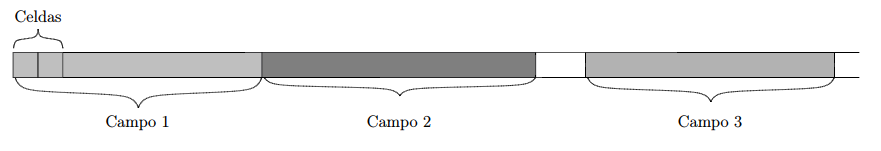
\includegraphics[width=0.8\textwidth]{./resources/specifiers.png}
                \caption*{Campos de escritura y lectura en una Línea de texto}
            \end{figure}
        \item Los especificadores más relevantes se explicarán a continuación:
    \end{itemize}
\end{frame}

\begin{frame}[fragile]{Formatos de representación de datos} 
  \textbf{Especificador de tipo Integer I\textit{n}}
    \begin{itemize}[<+(1)->] 
        \item El valor es representado en notación usual decimal.
        \item Si el valor es negativo, el signo - irá a la izquierda del primer dígito sin espacio de separación.
        \item Si se utilizan varios dígitos, estos ván juntos, sin espacios de separación y el primer dígito a la izquierda es diferente de 0.
        \item El dígito correspondiente a las unidades está ubicado en el extremo derecho de la cadena de caracteres utilizada.
        \item Los caracteres a la izquierda del primer dígito o eventualmente el signo - son espacios.
    \end{itemize}
\end{frame}

\begin{frame}[fragile]{Formatos de representación de datos} 
  \textbf{Especificador punto fijo de tipo Real F\textit{n.d}}
    \begin{itemize}[<+(1)->] 
        \item El valor es representado en notación usual decimal.
        \item En caso que el número sea negativo, el caracter - va a la izquierda de la parte entera o el punto (si la parte entera es 0), sin espacios.
        \item La parte fraccionaria del valor real ocupa los últimos $d$ caracteres del campo sin espacios, solamente dígitos (0-9), el caracter anterior a la parte fraccionaria corresponde al caracter punto “.”.
        \item Los dígitos de la parte entera del valor van a la izquierda del punto, sin espacios de separación. En caso que la parte entera sea diferente de 0, el primer dígito es diferente de 0; en el caso que la parte entera sea 0, el primer dígito es 0 o ningún caracter.
    \end{itemize}
\end{frame}

\begin{frame}[fragile]{Formatos de representación de datos} 
  \textbf{Especificador punto flotante de tipo Real (simple presición) E\textit{n.d}}
    \begin{itemize}[<+(1)->] 
        \item Las últimas cuatro plazas del campo están reservadas para el exponente, comienza con la letra E, seguido del signo + o del signo - y dos dígitos (0-9); es decir, por ejemplo E+09.
        \item La parte fraccionaria de la representación en punto flotante del valor real ocupan los $d$ caracteres del campo antes de la parte asignada al exponente sin espacios. Los caracteres asignados para la parte fraccionaria son únicamente dígitos (0-9).
        \item El caracter “.” va a la izquierda de la parte decimal, sin espacios.
        \item La parte entera está representada por 0 o níngun caracter y va a la izquierda del punto, sin espacios de separación.
        \item En caso que el número sea negativo, el caracter - va a la izquierda de la parte entera o el punto sin espacios.
        \item El \textbf{especificador punto flotante de tipo Real (doble presición) D\textit{n.d}} obedece a las anteriores reglas.
    \end{itemize}
\end{frame}

\begin{frame}[fragile]{Formatos de representación de datos} 
  \textbf{Especificador punto de tipo character A y A\textit{d}}
    \begin{itemize}[<+(1)->] 
        \item Se emplean para expresiones que pueden tomar distintos valores.
        \item En la escritura se puede asignar una cadena de caracteres de cierta longitud mediante '=' y entre comillas.
    \end{itemize}
 \onslide<4-> \textbf{Especificador punto de tipo logical L y L\textit{d}}
    \begin{itemize}[<+(2)->] 
        \item El especificador L utiliza un campo de dos caracteres mientras L\textit{d} uno para \textit{d} caracteres.
    \end{itemize}
\end{frame}

\begin{frame}[fragile]{Modificadores de formato}
   \begin{table}[]
    \centering
    \label{Tabla_especificaciones}
    \resizebox{10.55cm}{!} {
      \begin{tabular}{|l|l|l|}
        \hline
        \textbf{Esp.}   & \textbf{Nombre}                   & \textbf{Acción}                                                               \\ \hline    
        I\textit{n}     & Entero                            & Asigna un campo de $n$ caracteres para representar un entero en notación      \\          
                        &                                   & decimal, justificado por derecha.                                             \\ \hline
        F\textit{n.d}   & Punto fijo                        & Asigna un campo de $n$ caracteres para representar un real en formato punto   \\    
                        &                                   & fijo, con $d$ dígitos para la parte fraccionaria, justificado por la derecha. \\ \hline
        E\textit{n.d}   & Punto flotante                    & Asigna un campo de $n$ caracteres para representar un real en formato punto   \\  
                        &                                   & flotante, con $d$ dígitos para la parte fraccionaria, justificado por derecha.\\ \hline  
        D\textit{n.d}   & Punto flotante doble presición    & Lo mismo que especificador E, pero en doble presición.                        \\ \hline
        g\textit{n.d}   & Real                              & Asigna una campo de longitud $n$, con $d$ dígitos; dependiendo del valor:     \\     
                        &                                   & en punto fijo, justificación a la la izquierda o punto flotante,              \\
                        &                                   & justificación a la derecha.                                                   \\ \hline
        A\textit{n}     & Texto                             & Asigna un campo de longitud $n$, para expresiones de tipo $character$.        \\ \hline
        A               & Texto                             & Asigna un campo de longitud, la longitud de la expresión de tipo $character$. \\ \hline
        $\ldots$        & Texto fijo                        & Asigna el campo de longitud la cadena de caracteres y escribe en el campo .   \\
                        &                                   & la cadena.                                                                    \\ \hline
        L\textit{n}     & Lógico                            & Asigna un campo de $n$ caracteres para valores lógicos, justificación a       \\ 
                        &                                   & la derecha.                                                                   \\ \hline
        L               & Lógico                            & Asigna un campo de dos caracteres para valores lógicos, justificación por     \\ \hline 
                        &                                   & la derecha.                                                                   \\ \hline 
        X               & Espacio                           & Desplaza el siguiente campo de un espacio.                                    \\ \hline
        T\textit{n}     & Tabulador                         & El siguiente campo comienza en la columna $n$.                                \\ \hline
        \$              & Manteción de la línea             & No cambia la linea al final una instrucción de escritura o lectura.           \\ \hline
        /               & Cambio de línea                   & Cambia de línea.                                                              \\ \hline
      \end{tabular}}
          \caption*{Principales especificadores de formato y control}          
    \end{table}
\end{frame}



  %-----------------------------------------------------------------------------80
% SECTION TITLE|
%-----------------------------------------------------------------------------80

\section{Lectura y escritura de archivos}  

%-----------------------------------------------------------------------------80
% CONTENT
%-----------------------------------------------------------------------------80

\subsection{Apertura/Lectura y escritura de archivos}

\begin{frame}[fragile]{} 
    \begin{itemize}[<+(0)->]
        \item [] \textbf{} 
        \item 
        \vspace{0.1cm}
        \begin{minted}{bash}
        [softbutterfly\@SB-PC]$ programa    
        Introduzca los valores de la matriz A de talla 3x2
        1,2,3,4 5 6
        La matriz que usted ha introducido es:
        Primera Fila           1           4
        Segunda Fila           2           5
        Tercera Fila           3           6
        [softbutterfly\@SB-PC]  
        \end{minted}
    \end{itemize}
\end{frame}
  \input{sections/07_ejec_comand_fortran08}
  \input{sections/08_proyecto2_arch_config}
  
\end{document}